\documentclass{ieeeaccess}
% IEEE Access Topical Review. Template: ACCESS_latex_template_20260513 (official, ieeeaccess.cls).
% Build: bash build.sh   (pdflatex -> bibtex -> pdflatex x2)
\usepackage{cite}
\usepackage{amsmath,amssymb,amsfonts}
\usepackage{graphicx}
\usepackage{textcomp}
\usepackage{booktabs}
\usepackage{array}
\usepackage{url}
\makeatletter
\g@addto@macro{\UrlBreaks}{\do\-\do\_}
\makeatother
\graphicspath{{figures/}}
% Row spacing for the comparison tables (booktabs \addlinespace between entries).
\newcommand{\rowgap}{\addlinespace[2.5pt]}

\begin{document}
\history{Date of publication xxxx 00, 0000, date of current version xxxx 00, 0000.}
\doi{10.1109/ACCESS.2026.0000000}

\title{Beyond Exponential Decay: Rethinking Error Accumulation in Large Language Models}

% TODO(authors): confirm city/country for each address, middle initials, and IEEE membership if any.
\author{\uppercase{Mikhail L. Arbuzov}\authorrefmark{1},
\uppercase{Sisong Bei}\authorrefmark{2},
\uppercase{Ziwei Dong}\authorrefmark{3},
\uppercase{Dmitri Kalaev}\authorrefmark{4},
AND \uppercase{Alexey Shvets}\authorrefmark{5}}

\address[1]{Independent Researcher, CITY, COUNTRY (e-mail: mike.arbuzov54@gmail.com)}
\address[2]{Independent Researcher, CITY, COUNTRY (e-mail: qurining@gmail.com)}
\address[3]{Independent Researcher, CITY, COUNTRY (e-mail: ziwei.dong@alumni.emory.edu)}
\address[4]{Independent Researcher, CITY, COUNTRY (e-mail: kalaevdr@gmail.com)}
\address[5]{Palo Alto Networks, CITY, COUNTRY (e-mail: ashvets@paloaltonetworks.com)}
\tfootnote{TODO(authors): funding statement, e.g., ``This work received no external funding.''}

\markboth
{Arbuzov \headeretal: Beyond Exponential Decay}
{Arbuzov \headeretal: Beyond Exponential Decay}

\corresp{Corresponding author: Mikhail L. Arbuzov (e-mail: mike.arbuzov54@gmail.com).}

\begin{abstract}
A widely cited argument holds that large language models must fail on long outputs: if every generated token can derail the answer with a fixed, independent probability, the chance of a fully correct answer decays exponentially with length. This topical review examines the evidence on its two assumptions. On uniform risk across positions, studies of attention sparsity, cache and prompt compression, long-context perplexity, and generation-time uncertainty mostly find that a minority of positions carries the long-range information and the decisions an output depends on. That minority's size depends on the measure, and some studies find relevant content spread across whole reasoning traces. On independence, studies of error snowballing, self-conditioning, self-correction, and correlated mistakes show that errors depend on each other within an answer and are shared across samples and models; work on the geometry of internal representations, and on mapping representations between models, suggests why, but we found no study that links measured geometry to shared errors. We organize the evidence around a two-rate model in which reliability is set by the number and difficulty of key decisions rather than the number of tokens. The model predicts slow or bounded decay when decisions stay few and other positions add little cumulative risk, and it recovers exponential decay when every step adds new decisions, as we argue happens in long agentic tasks. We compare results within their settings, grade each line of evidence, identify where the argument fails, and propose a direct test of how key positions grow with length.
\end{abstract}

\begin{keywords}
Error accumulation, key tokens, large language models, long-context reliability, representation geometry, sparse attention, uncertainty quantification.
\end{keywords}

\titlepgskip=-21pt

\maketitle

% =====================================================================
\section{Introduction}
\label{sec:intro}
\PARstart{A}{utoregressive} language models, the argument goes, are doomed on long outputs: if every generated token has a fixed chance $e$ of leaving the set of correct answers, an answer of $n$ tokens is correct with probability $(1-e)^n$~\cite{lecun2023why}. At $e = 1\%$, a 100-token answer is fully correct only about 37\% of the time, and longer answers approach certain failure. Dziri et al.~\cite{dziri2023faith} prove step-level analogues for compositional tasks: when each step of a multi-step computation fails independently, or when a mistake is recovered from only with small probability, the probability of a correct final answer falls exponentially in the number of steps, toward a small floor set by the chance of reaching the right answer from a wrong path. LeCun drew a strong conclusion from the argument: training can make $e$ smaller but cannot remove the problem, and a solution would require models that are not autoregressive~\cite{lecun2023why}.

The argument rests on two assumptions: that risk is the same at every position, and that errors at different positions are independent. Evidence on both exists, but it sits in literatures that are reviewed separately and mostly for other ends, such as shrinking caches and prompts or quantifying uncertainty, and those reviews have not assembled it into a test of either assumption. The evidence as a whole has therefore not been weighed against the assumptions, and the answer now matters. Reasoning models write thousands of tokens before answering~\cite{cai2025rkv}, and agents are evaluated on software tasks graded by how long they take human experts~\cite{kwa2025measuring}. If reliability decayed exponentially with every token, such outputs would almost never be correct, and LeCun's conclusion would stand. Whether reliability does decay that way, and under which conditions, decides whether that conclusion follows and where anyone building on these models should spend effort on reliability. There are already reasons for doubt. Chain-of-thought prompting, in which few-shot exemplars show intermediate steps before the answer, raised the accuracy of PaLM 540B on grade-school math from 17.9\% to 56.9\%~\cite{wei2022chain}. That study changed the prompting strategy, not only the length, and scored final answers rather than error-free traces, so it is no controlled test of length; it does suggest that token count alone is a poor guide to reliability.

This review argues that both assumptions fail. Risk is not uniform across positions: a minority of positions carries the long-range information and the decisions an answer depends on. Nor are errors independent: an early wrong commitment is carried forward, and wrong answers agree across samples and across models. A two-rate model that counts decisions instead of tokens is consistent with this evidence. It also says where exponential decay returns: when every step of a task brings new decisions, as we argue happens in long agentic work. That both assumptions fail therefore does not rule out exponential decay; it shows that the argument cannot establish exponential decay as a general law of autoregressive generation.

The evidence is organized around three research questions, posed formally in Section~\ref{sec:framework}: whether a few positions carry the long-range information (RQ1, Section~\ref{sec:importance}), whether errors originate at a few hard decisions (RQ2, Section~\ref{sec:hardness}), and whether errors are independent (RQ3, Section~\ref{sec:dependence}). As a topical review, the paper makes five contributions:
\begin{itemize}
\item a single model that connects work on long-context sparsity, generation-time uncertainty, and error dependence, which are usually reviewed separately (Section~\ref{sec:framework});
\item comparison tables that report each result with the setting it holds in (Tables~\ref{tab:importance}, \ref{tab:hardness}, and \ref{tab:crossmodel});
\item worked calculations, using classical tools (the chain rule of probability, positive association, and majority voting), of how dependence between errors changes sequence-level reliability and the value of sampling several answers (Section~\ref{sec:dependence} and Appendix~\ref{app:derivations});
\item a reconciliation of apparently conflicting results, including agent evaluations that report exponential decay in task length (Section~\ref{sec:reconcile}); and
\item a graded assessment of the evidence and a set of open problems, including a protocol for measuring the growth of key positions directly (Sections~\ref{sec:reconcile} and~\ref{sec:open}).
\end{itemize}
An earlier version of this argument appeared as a preprint; this review revises it throughout, checks every cited result against its source, and adds the evidence published since. Section~\ref{sec:scope} describes the scope and method.

% =====================================================================
\section{Scope and Method of This Review}
\label{sec:scope}

\subsection{Question and Scope}
This review asks one question: what does the published evidence on large language models (LLMs) say about the assumptions behind exponential error accumulation? It covers work that measures, or builds systems on, one of three properties: which tokens carry the long-range information an output depends on; where generation errors originate; and whether errors at different positions, in different samples, or in different models are statistically dependent. Under the third heading it includes work on the geometry of internal representations and on mapping representations between models, because that work bears on why errors cluster. It excludes work on training-time scaling laws and taxonomies of hallucination that do not locate errors at positions in an output.

\subsection{How the Literature Was Assembled}
The starting point was the reference list of the first version of this argument, posted as a preprint in 2025~\cite{arbuzov2025beyond}. From those papers we followed citations backward and forward, and we searched arXiv, the ACL Anthology, and the proceedings of NeurIPS, ICML, ICLR, and the Conference on Language Modeling for work posted between 2015 and September 2026. Older work is cited where it supplies the mathematics or the precedent for a line of research (Appendices~\ref{app:derivations} and~\ref{app:adjacent}). Peer-reviewed work is preferred. When a preprint reports a measurement that no peer-reviewed work provides, it is included and cited as a preprint. The search was narrative rather than systematic: it aimed at the studies that bear most directly on the three questions, not at exhaustive coverage of each literature.

\subsection{How the Evidence Was Checked}
Every cited result was read in the full text at the passage the review relies on, with two exceptions recorded in the citation ledger described below: a classical inequality cited as a standard result, and one paywalled paper for which only the abstract was available. For a few works, a preprint, technical report, or author manuscript was read in place of the published version. The ledger records, for each citing sentence, the supporting passage, its location in the source, and the setting in which the result holds: the models, data, and task. Where only the abstract was accessible, the citing sentence claims no more than the abstract does. Venues were confirmed on the publisher's or the conference's own pages. Numbers in the comparison tables are reported as their authors state them, together with the setting they apply to; this review runs no new experiments. The grades in Table~\ref{tab:strengths} are the authors' judgment, based on how many independent groups and methods support a claim, whether the support is direct or inferred, and the scale of the models tested. The ledger is available as supplementary material.

\subsection{Relation to Existing Reviews}
Recent reviews each cover one of the mechanisms discussed here, usually as an efficiency or control technique. Surveys of key--value cache management~\cite{li2025kvsurvey} and of prompt compression~\cite{li2024promptsurvey} catalog ways to shrink the cache or the prompt. A review of uncertainty quantification~\cite{zhang2026activeuq} tracks how uncertainty is now used as an active control signal, for example to allocate test-time computation. A review of latent communication~\cite{liu2026latentsurvey} classifies ways for models to exchange internal states instead of text. The uncertainty review notes that early mistakes can derail a chain of thought and surveys methods that propagate uncertainty across agent steps. But none of these reviews models how the findings compose into the probability that a long output is correct, the question this review is organized around. A companion paper~\cite{arbuzov2026architecture} develops the intervention side of the question: how the recurring failures at key decisions can be cataloged and targeted inside a deployment domain.

Appendix~\ref{app:adjacent} places the review against older and adjacent lines of work that it does not survey in full: compounding error and recovery, from imitation learning and exposure bias to self-correction; attention, intervention, uncertainty, and verification as ways to find the positions that matter; uneven computation across tokens; voting with correlated voters; and the comparison of representations across networks, including probes for truth. Much of the machinery used here has precedent there, from the quadratic bound on compounding error to the jury theorem and the failure of independence among independently written programs. What this review adds is the assembly: one model that connects these findings to the probability that a long answer is correct, a reading of the evidence against that model's parameters, and the measurements still needed to test it.

% =====================================================================
\section{A Simple Model of Sequence-Level Error}
\label{sec:framework}
This section sets the uniform model beside a two-rate model in which reliability is set by how many hard decisions an answer contains, not by how many tokens it has, provided that the total risk at the other positions stays bounded.

\subsection{The Uniform Model}
The uniform argument fits in a few lines. Suppose every generated token can derail the answer with the same small probability $e$, independently of every other token. The chance that an answer of $n$ tokens contains no such error is then
\begin{equation}
\label{eq:uniform}
P_{\text{uniform}}(\text{correct}) = (1-e)^{n},
\end{equation}
which falls exponentially with length. A model that gets $99\%$ of its tokens right ($e = 0.01$) would complete a 2{,}000-token answer without error about twice in a billion attempts.

Throughout this review, a token counts as an \emph{error} only if it commits the answer to something wrong: a false fact, an invalid step, the wrong referent. A synonym, a reordered clause, or a different but valid derivation step is not an error in this sense.

With that definition fixed, \eqref{eq:uniform} rests on two assumptions: every position is equally likely to fail, and failures at different positions are independent. Sections~\ref{sec:importance}--\ref{sec:dependence} examine the evidence on each assumption. A third premise, that an error once made is never repaired, is one this review largely accepts: the evidence in Section~\ref{sec:dependence} shows that models seldom repair early errors without outside help, although models trained to reason or to correct themselves partly do. The two-rate model below keeps it, and so describes the probability of an error-free answer. Most of the studies reviewed score final answers instead, which can be right even after a repaired mistake; their results bear on the model's premises rather than test its predictions.

Independence is the subtler of the two. Written exactly, the probability of an error-free answer is $\prod_{t=1}^{n}(1-h_t)$, where $h_t$, the \emph{hazard} at position $t$, is the probability of an error there given that none has occurred before it. This identity needs no independence, and \eqref{eq:uniform} follows whenever every $h_t$ equals $e$. Independence matters when $e$ is taken to be a per-token error rate measured over whole outputs, a rate that also counts tokens written after an earlier error. If an earlier error makes later ones more likely, that rate overstates the risk at a position whose prefix is still correct, and when the rate is the same at every position, \eqref{eq:uniform} understates the chance of a correct answer (Appendix~\ref{app:union}).

\subsection{The Two-Rate Model}
Suppose instead that a small set of $k$ positions carries the decisions that determine correctness: which fact to state, which branch of a derivation to take, which entity a pronoun refers to. Call these \emph{key positions}, each failing with probability $e_{\text{key}}$. The remaining $n-k$ positions are constrained by syntax and by what has already been written; position $i$ among them fails with a much smaller probability $e_{\text{non}}(i)$ that shrinks as context accumulates. If failures are still treated as independent, the probability of a correct answer becomes
\begin{equation}
\label{eq:tworate}
P(\text{correct}) \approx (1-e_{\text{key}})^{k} \prod_{i=1}^{n-k} \bigl(1-e_{\text{non}}(i)\bigr).
\end{equation}
The uniform model is the special case $k = n$.

\emph{Running example.} Take the same 2{,}000-token answer, but let it contain $k = 20$ key decisions, each failing with probability $e_{\text{key}} = 0.05$, while the other positions fail with $e_{\text{non}}(i) = 0.02\, i^{-1.5}$. Equation~\eqref{eq:tworate} gives $P(\text{correct}) \approx 0.34$. Lowering the key-decision error rate to $0.02$ raises it to about $0.63$; adding another thousand predictable tokens barely changes it. Under this model, reliability is set by how many hard decisions an answer contains and how often each one goes wrong, not by how long the answer is. The parameters are illustrative, not measured; Section~\ref{sec:open} describes how they could be measured.

\subsection{How the Number of Key Positions Grows}
What happens as answers get longer depends on how $k$ grows with $n$. Table~\ref{tab:regimes} lists four cases. The first three are the regimes the original version of this argument considered; the fourth recovers exponential decay and is the case to watch in long multi-step tasks, where every new subtask brings new decisions (Section~\ref{sec:reconcile}).

\begin{table}[!t]
\caption{How the growth of key positions $k(n)$ shapes sequence-level reliability under \eqref{eq:tworate}, assuming the non-key factor stays bounded away from zero. Here $\lambda = \ln\bigl(1/(1-e_{\text{key}})\bigr) \approx e_{\text{key}}$ (Appendix~\ref{app:regimes}).}
\label{tab:regimes}
\centering
\footnotesize
\renewcommand{\arraystretch}{1.15}
\begin{tabular}{@{}>{\raggedright\arraybackslash}p{1.65cm}>{\raggedright\arraybackslash}p{2.6cm}>{\raggedright\arraybackslash}p{3.4cm}@{}}
\toprule
\textbf{Growth of $k$} & \textbf{Decay of $P(\text{correct})$} & \textbf{Reading} \\
\midrule
$k \sim c\ln n$ & power law, $n^{-c\lambda}$ & slow; small exponent when $e_{\text{key}}$ is small \\
$k \sim \sqrt{n}$ & stretched exponential & faster, still far slower than \eqref{eq:uniform} \\
$k \to k_{\max}$ & constant in $n$ & a fixed decision budget; added length costs only non-key risk \\
$k \propto n$ & exponential, rate $\propto e_{\text{key}}$ & uniform behavior returns at a lower rate \\
\bottomrule
\end{tabular}
\end{table}

Figure~\ref{fig:regimes} plots the first three cases, with the uniform model for comparison, for the running example's parameters.

\begin{figure}[!t]
\centering
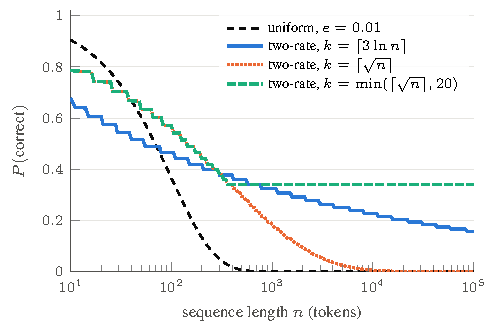
\includegraphics[width=\columnwidth]{fig1_decay_regimes}
\caption{Sequence-level correctness under the uniform model \eqref{eq:uniform} and under the two-rate model \eqref{eq:tworate} for three growth laws of $k$. Parameters are illustrative: $e = 0.01$; $e_{\text{key}} = 0.05$; $e_{\text{non}}(i) = 0.02\, i^{-1.5}$. The curves show functional forms, not fits to data.}
\label{fig:regimes}
\end{figure}

Table~\ref{tab:regimes} assumes that the non-key factor of \eqref{eq:tworate} stays bounded away from zero. That holds only if the non-key error rates are summable, $\sum_i e_{\text{non}}(i) < \infty$, as with any rate bounded by $c\, i^{-p}$ for some $p > 1$ (Appendix~\ref{app:nonkey}). A constant rate, however small, does not qualify: at $e_{\text{non}} = 10^{-4}$ per token, the non-key factor is about $0.82$ for a 2{,}000-token answer but about $0.14$ at 20{,}000 tokens and $5\times10^{-5}$ at 100{,}000. The claim that predictable tokens become more predictable as context accumulates is therefore load-bearing.

\subsection{What the Model Asks of the Evidence}
The model turns one question about length into three questions about structure, which organize the rest of this review. The first two test the model's two premises about the key positions themselves: that few positions carry the information an answer depends on, and that errors originate at few decisions. The third concerns the independence that \eqref{eq:tworate} still assumes. If failures are correlated, the picture changes in two directions: failures cluster within one answer, and sampling several answers recovers less.
\begin{itemize}
\item \textbf{RQ1, importance.} Do only a few positions carry the long-range information an answer depends on (Section~\ref{sec:importance})?
\item \textbf{RQ2, hardness.} Do errors originate at a few uncertain decision points rather than uniformly (Section~\ref{sec:hardness})?
\item \textbf{RQ3, dependence.} Are errors at different positions, and in different samples or models, independent (Section~\ref{sec:dependence})?
\end{itemize}
Importance and hardness are two different empirical handles on the key positions of \eqref{eq:tworate}: one asks where information flows, the other where mistakes are made. They need not pick out the same tokens. A name copied from far back in the context needs distant information but involves no real choice; a token at which the outcome forks involves a choice that may need no distant information at all. Section~\ref{sec:open} asks how far the two coincide.

\begin{table*}[!t]
\caption{Reported shares of positions that carry the signal, by criterion. Numbers are as stated by the original authors, in the settings given; they measure different things and are not directly comparable.}
\label{tab:importance}
\centering
\footnotesize
\begin{tabular}{@{}>{\raggedright\arraybackslash}p{2.6cm}>{\raggedright\arraybackslash}p{5.0cm}>{\raggedright\arraybackslash}p{5.0cm}>{\raggedright\arraybackslash}p{3.9cm}@{}}
\toprule
\textbf{Study} & \textbf{Criterion} & \textbf{Setting} & \textbf{Reported share} \\
\midrule
Fang et al.~\cite{fang2024what} & Prediction improves by more than 2 nats with the full context versus a truncated short context & GovReport; one corpus, teacher forced & fewer than 10\% of tokens \\
\rowgap Vakilian et al.~\cite{vakilian2025short} & Last 64--96 tokens reproduce a confident top-1 prediction (or the whole distribution) & 7--8B models; prefixes up to about 7{,}000 tokens & 75--80\% of confident positions (32--45\% for the whole distribution, LLaMA-3) \\
\rowgap Quest~\cite{tang2024quest} & Cached tokens skippable at decode time with negligible perplexity change & LongChat-7B, PG19; layers after the second & more than 90\% skippable \\
\rowgap H2O~\cite{zhang2023h2o} & Cache budget, half high-attention and half recent tokens, matching full-cache accuracy & OPT, LLaMA, GPT-NeoX; mostly short-answer tasks & 20\% of the sequence \\
\rowgap PyramidKV~\cite{cai2024pyramidkv} & Prompt cache matching full-cache scores & LongBench, prompts of about 1--18K tokens & about 12\% (2{,}048 entries) \\
\rowgap R-KV~\cite{cai2025rkv} & Decode-time cache of the model's own reasoning matching full-cache accuracy & Two distilled reasoning models; MATH-500, AIME-24 & 10--54\% of the generated length \\
\rowgap LLMLingua~\cite{jiang2023llmlingua} & Prompt tokens kept with about 1.5-point loss & GPT-3.5-Turbo; few-shot GSM8K & up to 20$\times$ compression (larger losses on BBH) \\
\rowgap TextFooler~\cite{jin2020textfooler} & Words a synonym attack changes to flip a classifier & Text classification and entailment & 3.5--22\% by dataset and model (lowest on IMDB, highest on AG News) \\
\bottomrule
\end{tabular}
\end{table*}

% =====================================================================
\section{RQ1: Token Importance}
\label{sec:importance}

\emph{Claim.} At any step of generation, a minority of earlier positions carries most of the information the model uses. How small the minority is depends on how importance is measured, and which positions belong to it changes with the query and with the step.

\subsection{Evidence}
Models do not use long contexts uniformly: accuracy is often highest when the relevant information sits at the beginning or end of the prompt and lowest when it sits in the middle~\cite{liu2023lost}. Beyond such position effects, three kinds of study point the same way, and Table~\ref{tab:importance} lists them with the settings in which each number holds.

The most direct evidence asks which predictions need distant context at all. Early studies already pointed the same way. An LSTM language model used about 200 tokens of context on average, and shuffling the words more than 50 tokens back left its loss unchanged, although replacing those distant words with unrelated text did raise it~\cite{khandelwal2018sharp}. On PG-19 books, two Transformer language models that accept 8K tokens (a Routing Transformer and a local-attention variant of it) gained essentially nothing in overall perplexity from context more than 2K tokens back; the gains, mainly in the Routing Transformer, were confined to small subsets of tokens, such as rare tokens and tokens that can be copied from the distant context~\cite{sun2021longrange}. Fang et al.~\cite{fang2024what} compare each token's likelihood under the full context with its likelihood under a truncated short context; on the GovReport corpus, fewer than one token in ten gains more than 2 nats of log-probability from the longer context. The window behind that figure is not stated, and the result comes from one corpus. Vakilian et al.~\cite{vakilian2025short} ask the converse question for positions a model already predicts correctly and confidently. For 75--80\% of them, the last 64--96 tokens reproduce the full-context prediction, although for LLaMA-3 the share falls to 32--45\% when the whole next-token distribution, rather than only the top choice, must match.

A second line of work measures attention and keeps only the positions it favors. Decode-time attention in LongChat-7B is so concentrated that an oracle selector can skip more than 90\% of cached tokens in every layer after the second with negligible change in perplexity~\cite{tang2024quest}. In a 128K-token context, attention computed from only the top-$k$ positions approaches full attention once $k$ is in the low hundreds, which lets 8B-parameter models serve such contexts on a single consumer graphics card by attending at each step to about a hundred retrieved positions plus a fixed set of initial and recent ones~\cite{liu2024retrieval}. On most of the benchmarks tested, full-cache accuracy is matched by prompt caches cut to roughly a tenth of their length~\cite{li2024snapkv,cai2024pyramidkv}, or by caches limited to a fifth of the sequence and split between high-attention and recent tokens~\cite{zhang2023h2o}. One model was trained from the start with sparse attention, which keeps a compressed coarse view of all earlier positions alongside a few selected blocks and a local window; in the authors' single-run comparison, it matched or exceeded a full-attention twin~\cite{yuan2025nsa}. It reads only a minority of positions in full but removes none.

The third line removes tokens outright. Few-shot reasoning prompts can be compressed severalfold by dropping predictable tokens~\cite{jiang2023llmlingua}. A model continually pre-trained to fold each demonstration into a single anchor token cut the cache of five-shot prompts by up to 99\% on short question-answering benchmarks at an average accuracy cost of about 1.5\%~\cite{pang2024anchor}. Closest to this review's setting, R-KV compresses a reasoning model's own chain of thought during generation and matches full-cache accuracy with a cache of a tenth to about half of the generated length, depending on the model and benchmark~\cite{cai2025rkv}.

\begin{table*}[!t]
\caption{Studies that locate errors at a minority of decision points or act on them. Numbers are as stated by the original authors, in the settings given.}
\label{tab:hardness}
\centering
\footnotesize
\begin{tabular}{@{}>{\raggedright\arraybackslash}p{2.7cm}>{\raggedright\arraybackslash}p{4.2cm}>{\raggedright\arraybackslash}p{4.6cm}>{\raggedright\arraybackslash}p{5.0cm}@{}}
\toprule
\textbf{Study} & \textbf{How decision points are found} & \textbf{Setting} & \textbf{Reported result} \\
\midrule
Bigelow et al.~\cite{bigelow2025forking} & Re-sampling at each token & GPT-3.5, seven tasks & Abrupt outcome shifts in up to 63\% of examples \\
\rowgap Lin et al.~\cite{lin2024critical} & Rollouts after each token of a wrong trace & Llama-3-8B; 100 wrong traces each from GSM8K and MATH training sets & One critical token per trace; replacing it recovers about 30\% (one re-sample) and over 90\% (within 64) \\
\rowgap Wang et al.~\cite{wang2025beyond8020} & Entropy, top 20\% (authors' cutoff) & Qwen3 8B to 32B, reinforcement learning on math & Over half of tokens below 0.01 entropy; training on the top 20\% matches or beats full training \\
\rowgap He et al.~\cite{he2025adadec} & Entropy above a learned threshold & Nine 0.6--8B code models & Look-ahead at about 7\% of steps: +3.6 to +7.6 points on average per benchmark \\
\rowgap Li et al.~\cite{li2025egb} & Entropy above a threshold, with a verifier & Six 1--8B models, math and finance & +18\% (relative) over single-path decoding; 31--75\% faster than beam search \\
\rowgap Zheng et al.~\cite{zheng2025processbench} & Expert consensus on the first error & 3{,}400 solutions, mostly competition math & Most first errors fall in the opening steps \\
\bottomrule
\end{tabular}
\end{table*}

\subsection{Limits}
Three findings narrow what this evidence shows.

\emph{The important set moves.} Which prompt positions matter changes with the instruction~\cite{li2024snapkv} and with the query~\cite{tang2024quest}, and over long generations the distribution of importance itself shifts~\cite{li2025scbench}. Methods that compress the context for the current query do well on that query and lose accuracy on follow-up queries about the same context~\cite{li2025scbench}. Sparsity holds at each step; a fixed small subset does not.

\emph{High attention is not the same as carrying content.} The first token of a sequence often absorbs attention that contributes little to the value computation, a sink that emerges during pre-training~\cite{gu2025sink}, and in the attention maps shown by the PyramidKV authors, the few tokens on which upper layers concentrate are such sinks~\cite{cai2024pyramidkv}. On long chains of thought, selection by attention alone fell well short of selection that also removes redundancy~\cite{cai2025rkv}. Eviction policies applied to instructions could not tell which entries were safe to drop~\cite{chen2026pitfalls}.

\emph{Aggressive compression breaks reasoning first.} With 40\% or more of the cache kept, retrieval and reasoning tasks were both stable; at about 20--30\% or less, multi-step arithmetic and code degraded sharply while retrieval-oriented tasks held up comparatively well~\cite{liu2026semantic}. Under prompt compression, some instructions came to be ignored entirely and protected system prompts leaked~\cite{chen2026pitfalls}. A fixed window of a few initial tokens plus recent ones keeps perplexity stable over millions of tokens, but anything outside the window is lost~\cite{xiao2024streamingllm}.

\subsection{What This Means for the Model}
The evidence supports the first premise of \eqref{eq:tworate} on the side of information: at each step, the information an answer depends on sits in a minority of earlier positions, so the positions whose content must be read correctly at any step are far fewer than $n$. Because that set changes from step to step, a long generation may still read many positions in all: the evidence motivates uneven risk across positions but does not estimate $k$. It does not support a single fixed fraction either. Reported shares run from under a tenth to more than half, depending on the criterion, the task, and whether the tokens belong to the prompt or to the model's own output. Importance also says where information flows, not where mistakes are made; whether errors concentrate at the same few positions is the question of Section~\ref{sec:hardness}.

% =====================================================================
\section{RQ2: Token Hardness}
\label{sec:hardness}

\emph{Claim.} Errors originate disproportionately at a minority of decision points, where one choice redirects the rest of the output, and spending extra computation at those points pays off. Not every error is found this way: some are made with high confidence, and some build up over a whole trace.

\subsection{Evidence}
The cleanest evidence comes from re-sampling a generation at one position and watching the outcome. Re-sampling GPT-3.5 outputs token by token on seven tasks, Bigelow et al.~\cite{bigelow2025forking} found \emph{forking tokens}, sometimes a single punctuation mark, at which the outcome shifts abruptly. Such shifts appeared in up to 63\% of examples depending on the task, alongside smaller effects that accumulate gradually along most paths. In 100 incorrect reasoning traces of Llama-3-8B from each of the GSM8K and MATH training sets, Lin et al.~\cite{lin2024critical} located a \emph{critical token} in all but one trace; forcing a different token at that one position recovered the correct answer in about 30\% of single re-samples and in over 90\% of cases within 64. The very first token can be such a position: when decoding branched over the ten most likely first tokens and then continued greedily, the most confident path contained a chain of thought for 88 of the first 100 GSM8K questions checked by hand, although no prompt asked for one~\cite{wang2024chain}. At the level of sentences, in work its authors call preliminary, re-sampling each sentence of distilled R1 reasoning traces 100 times on 20 MATH problems shows that a few sentences, mostly plan-generation and uncertainty-management steps, have outsized counterfactual influence on the final answer~\cite{bogdan2025anchors}. The Phi-4 report observes that correctness often hinges on a few such \emph{pivotal} tokens and trains on them directly, with preference pairs that differ in a single token~\cite{abdin2024phi4}.

Generation-time entropy is sharply skewed. Over half of all tokens in chain-of-thought generation by Qwen3-8B have entropy below 0.01; restricting policy-gradient updates to the 20\% of tokens with the highest entropy---a cutoff the authors chose---matched full-gradient reinforcement learning at 8B and exceeded it at 14B and 32B~\cite{wang2025beyond8020}. In DeepSeek-Coder-6.7B's failed HumanEval solutions, the steps where program logic first goes wrong carry far higher entropy than other steps (median 1.26 against 0.03), and an initial manual inspection found the correct token there usually ranked second or third rather than absent~\cite{he2025adadec}. Token difficulty is uneven at training time as well: in continual pretraining of a 1B-parameter model on mathematical text, only about a quarter of tokens showed a marked drop in loss, while about half were already learned~\cite{lin2024rho1}. Experts who annotated 3{,}400 math solutions, mostly to competition problems, located the earliest erroneous step, and most first errors fall in the opening steps. Short solutions and a constant per-step error rate would also produce that pattern, and about 30\% of candidate solutions were set aside because experts could not agree~\cite{zheng2025processbench}.

Acting on these points helps, as Table~\ref{tab:hardness} shows. Pausing for a short look-ahead only at high-entropy steps, a small fraction of all steps, raises code-generation pass rates over greedy decoding and beats beam search of the same width~\cite{he2025adadec}. In a verifier-guided beam search, branching only where entropy is high raises accuracy over single-path decoding across six models and five benchmarks while running faster than uniform beam search~\cite{li2025egb}. On our reading of the paper's own results table, though, uniform verifier-guided beam search already achieves most of that gain. Allocating test-time computation per prompt by estimated difficulty let a smaller model outperform one about 14 times its size in a FLOPs-matched comparison on MATH, on questions where it had a non-trivial success rate~\cite{snell2024scaling}. Redundant tokens can be dropped too: after fine-tuning on chains of thought pruned of tokens that an external classifier rated unimportant, Qwen2.5-14B-Instruct wrote about 40\% fewer reasoning tokens on GSM8K at a cost of 0.4 accuracy points, although smaller models and harder problems lost more~\cite{xia2025tokenskip}.

\subsection{Limits}
\emph{Uncertainty does not find every hard decision.} In one worked example, the Phi-4 report shows that pivotal tokens are not the same as low-probability tokens~\cite{abdin2024phi4}. In short-answer question answering, 16--47\% of wrong answers from instruction-tuned models place substantial probability on the correct answer's first tokens at the moment of answering, and most of these begin correctly and go wrong on later tokens~\cite{yeom2026commit}. Across 500 one-sentence answers from one model, correct and wrong alike, the step with the highest entropy coincided with the step at which the answer itself is emitted in only about a fifth of cases~\cite{yeom2026commit}. Some wrong answers are produced with high certainty even when the model demonstrably knows the right one, although such cases are a small fraction of all hallucinations~\cite{simhi2025choke}. Supervised probes on hidden states localize hallucinated entities in long outputs much better than token entropy: on Llama-3.3-70B, the area under the receiver operating characteristic curve is 0.87--0.90 against about 0.71~\cite{obeso2025entities}.

\emph{Some failures are spread out.} In 9 of 23 model and benchmark settings, the signal that predicts failure from a reasoning trace kept growing to the end of the trace; in the other 14, an early prefix predicted failure better than the full trace, although in most of these the advantage lay within statistical uncertainty~\cite{thoria2026fail}. For compressing reasoning traces, choosing sentences by entropy was no better than choosing them at random, and the authors conclude that the task-relevant content is not concentrated in a small set that such a heuristic can find~\cite{candussio2026demyst}. That study concerns where task information sits, not where errors arise. The forking-token study itself found gradual hazards along most paths alongside the abrupt ones~\cite{bigelow2025forking}.

\subsection{What This Means for the Model}
The second premise of \eqref{eq:tworate} is also supported: the outcome turns on a minority of decisions, and targeting them is effective. These studies locate where outcomes are sensitive, not where errors begin. Most of the critical tokens Lin et al.\ found did not coincide with the tokens where the error would conventionally be located~\cite{lin2024critical}, and none of the studies estimates $k$ or the hazard at the positions it finds. The evidence also qualifies the premise in two ways. First, $e_{\text{key}}$ is a property of decisions, not of high-entropy tokens; uncertainty is a useful but incomplete way to find them. Second, some failures do not localize, which is the case in which the non-key factor of \eqref{eq:tworate} matters most. Whether the positions that carry long-range information (Section~\ref{sec:importance}) are the same positions that decide the outcome has been tested only at the level of sentences. In distilled R1 reasoning traces, the sentence types that later sentences attend to most, through specialized ``receiver'' heads, are the types with the greatest counterfactual influence on the answer, a comparison the authors note is confounded by sentence position~\cite{bogdan2025anchors}. We found no study that makes the comparison at the level of tokens, or for the positions where errors originate; Section~\ref{sec:open} returns to this question.

% =====================================================================
\section{RQ3: Error Dependence and Representation Structure}
\label{sec:dependence}

\emph{Claim.} Errors are not independent. Within one answer, an early wrong commitment tends to be carried forward rather than corrected; across samples and across models, wrong answers agree more often than chance. Studies of internal representations suggest why: concepts occupy structured regions and directions that different models partly share. The behavioral evidence is direct; the geometric explanation is an interpretation the evidence supports but does not establish.

\subsection{Dependence Within One Answer}
The worry that errors compound is older than large language models: a model trained to predict each token from the true preceding tokens must, at inference time, condition on its own outputs, so errors can accumulate along the generated sequence~\cite{bengio2015scheduled}. When a model commits early to a wrong answer, later tokens tend to justify it. Asked to answer first, GPT-3.5, GPT-4, and LLaMA-2-70B-chat commit to yes or no within the first few tokens and, when that answer is wrong, usually support it with false claims. Yet the same model, shown each false claim in a fresh session, rejects most of them: on average from two-thirds to more than nine in ten, depending on the model~\cite{zhang2024snowball}. Long-horizon execution shows the same effect at the level of steps: per-step accuracy falls as a task proceeds, partly because models become more likely to err when their context contains their own earlier mistakes, an effect that models trained to reason before answering largely avoid~\cite{sinha2025illusion}.

\begin{table*}[!t]
\caption{Evidence that representations or errors are shared across models. The \emph{Models} column notes whether the evidence comes from encoders and embedding models or from generative LLMs.}
\label{tab:crossmodel}
\centering
\footnotesize
\begin{tabular}{@{}>{\raggedright\arraybackslash}p{2.9cm}>{\raggedright\arraybackslash}p{4.1cm}>{\raggedright\arraybackslash}p{4.6cm}>{\raggedright\arraybackslash}p{4.9cm}@{}}
\toprule
\textbf{Study} & \textbf{Models} & \textbf{What is shared} & \textbf{Caveat} \\
\midrule
Moschella et al.~\cite{moschella2023relative} & Small encoders, word embeddings, graph networks & Angles to anchor samples, approximately & Same-data retrainings strongest; stitching costs accuracy \\
\rowgap Maiorca et al.~\cite{maiorca2023translation} & Pretrained text and image encoders & Largely orthogonal maps between latent spaces & Needs hundreds to thousands of paired anchors \\
\rowgap Jha et al.~\cite{jha2025vec2vec} & Text-embedding models & Translatable embedding spaces without paired data & Unstable for unrelated backbones \\
\rowgap Huh et al.~\cite{huh2024platonic}; Gr\"oger et al.~\cite{groger2026aristotelian} & Vision and language models & Nearest-neighbor structure over paired data & Global convergence largely vanishes after calibration \\
\rowgap Ramesh and Li~\cite{ramesh2025activations} & LLMs, mostly one family & Activations usable by another model & Cross-family test covers two tasks \\
\rowgap Fu et al.~\cite{fu2026c2c} & LLMs across families & Key--value caches via a trained fuser & Fuser trained per pair; a self-paired fuser gives 70--90\% of its gain over a fine-tuned receiver \\
\rowgap Kim et al.~\cite{kim2025correlated} & 71 LLMs (HELM) & Same wrong option about 60\% of the time when both are wrong & Conditional on both being wrong; multiple choice \\
\rowgap Goel et al.~\cite{goel2025think} & 130 open LLMs & More similar mistakes with rising capability & Correlational; multiple choice \\
\bottomrule
\end{tabular}
\end{table*}

For models without trained reasoning, recovering from such a commitment is hard without outside help. Prompting 2023-era models to review and revise their answers on reasoning benchmarks did not improve accuracy and often lowered it, with correct answers changed to incorrect ones more often than the reverse~\cite{huang2024cannot}. When an identical error is placed in the model's own turn rather than the user's, open non-reasoning models correct it far less often, although the size of this gap reflects a controlled design with injected errors, and reasoning models largely do not show it~\cite{tsui2026blindspot}.

Training changes the picture. Multi-turn reinforcement learning on a model's own correction attempts turned the change from first to second attempt of Gemini 1.5 Flash on MATH500 from $-11.2$ to $+4.4$ points~\cite{kumar2025score}. With rewards that checked only final answers, reinforcement learning produced reasoning that includes verification and reflection on earlier steps~\cite{deepseek2025r1}. Finding the error is the harder half. Language models located the first logical mistake in reasoning traces poorly, at best 53\% overall accuracy, yet when one model was told where its mistake was and re-generated that step, 18--44\% of its wrong answers became correct, depending on the task~\cite{tyen2024llms}. Across the turns of a conversation, models that receive a task's requirements piecemeal often commit early to assumptions and attempt full solutions, then lean on those attempts instead of recovering, although the authors attribute most of the resulting drop in scores to greater variability between runs~\cite{laban2025lost}.

The same propagation appears when models pass internal states instead of text. In an audit that swapped relayed key--value caches between examples, receiving agents (copies of the same model as the sender) followed the content of a mismatched cache in about 64\% of cases, against about 22\% under a matched control~\cite{cheng2026audit}. A wrong state, once handed over, is acted on.

\subsection{Structure of Internal Representations}
Several lines of work find that models organize information in structured, low-dimensional ways. Truth and falsehood of simple factual statements are linearly represented in sufficiently large LLaMA-2 models, and shifting activations along the identified direction can make a model label false statements as true~\cite{marks2024geometry}. Binary concepts can be formalized as directions in a model's final-layer representations, with a ``causal'' inner product that unifies the senses in which they are linear~\cite{park2024linear}, and categorical concepts appear as polytopes in the final-layer representation, with hierarchy encoded as orthogonality~\cite{park2025categorical}. In small transformers trained on sequences from simple hidden Markov models, the residual stream linearly encodes the optimal belief state over the hidden states, though whether models trained on natural language carry comparable structure is untested~\cite{shai2024belief}. When a mixture of dictionary-learning experts with a preset number of strata is fitted to the final-layer embeddings of whole inputs, in models of up to 1.5B parameters, the strata differ in intrinsic dimension and align with the source of the data~\cite{li2025unraveling}. A statistical test on the input-embedding spaces of four open LLMs rejects local smoothness around some tokens, evidence against a single smooth manifold that is, on our reading, compatible with a stratified space~\cite{robinson2025token}. Across prompts of fixed length, those whose token representations occupy lower-dimensional point clouds have lower average surprisal~\cite{viswanathan2024geometry}.

Internal states also carry information about errors before or despite the output. Truthfulness signals concentrate at the tokens that state the answer, and a probe on the model's own activations can pick the correct answer out of its sampled candidates even when the model usually generates a wrong one~\cite{orgad2025know}. A probe can locate the needed information in the hidden states of a long-context model even when the generated answer is wrong~\cite{gao2024insights}. In reasoning models, a light probe at the end of each reasoning chunk predicts whether that chunk's intermediate answer is correct, and used as an early-exit test on one model it cut generated tokens by about a quarter at roughly unchanged accuracy~\cite{zhang2025reasoningprobe}. In the Qwen-3 family, the 14B model, and in nascent form the 4B and 8B models, have internal features that represent a word before it is generated and shape the token that precedes it, while the smallest models seldom have such features; even at 14B, planning more than a token ahead is rare~\cite{hanna2026planning}.

On our reading, this structure is what separates errors at non-key positions from errors at key positions (Section~\ref{sec:framework}): a slip that stays within the region of the current commitment is absorbed, while a wrong key decision moves the state to a different region, after which later tokens are locally coherent and globally wrong. The cited studies do not test this reading. They establish that structure exists and that errors are visible in it---not that the structure governs how errors spread.

\subsection{Shared Structure Across Models}
Whether this structure belongs to one model's training or to the data is a further question. Representations of independently trained networks can be mapped onto one another. Table~\ref{tab:crossmodel} summarizes the evidence. Angles between encodings are approximately preserved across retrainings and across architectures, which allows an encoder from one model to be stitched to a decoder trained on these anchor-relative representations of another, at some cost in accuracy~\cite{moschella2023relative}. The latent spaces of different pretrained text and image encoders are related by largely orthogonal maps, fitted from a few hundred to a few thousand paired samples~\cite{maiorca2023translation}. Without any paired data, the embedding spaces of different text-embedding models can be translated, although training is unstable for unrelated backbones~\cite{jha2025vec2vec}.

Most of this mapping evidence concerns encoders and embedding models rather than the hidden states of generative LLMs. Studies that include LLMs find that more capable language and vision models induce increasingly similar nearest-neighbor structure over paired data~\cite{huh2024platonic}. Once similarity scores are corrected for model width and depth, however, apparent global convergence largely disappears and only agreement on which inputs are each other's nearest neighbors persists~\cite{groger2026aristotelian}. Splicing an activation from one LLM into another's forward pass outperformed text-based debate on several tasks, mostly between two models of one family~\cite{ramesh2025activations}. A fuser trained separately for each pair can project one model's key--value cache into another's across families, improving accuracy over text hand-off by about three to five points~\cite{fu2026c2c}.

These results come with cautions. In the fuser's own ablation, pairing the receiver with a copy of itself already gave 70--90\% of the improvement that a different model gave over a fine-tuned receiver alone, although the authors read the remaining margin as the other model's contribution~\cite{fu2026c2c}. Latent collaboration between agents that are all copies of one model~\cite{zou2026latentmas} says nothing about different models. The audit cited above detected no example-specific transfer through one released cross-model projector on a synthetic task, a detection-level result that does not test that system's reported gains~\cite{cheng2026audit}. A commercial effort to bridge the hidden states of different models has also been announced.\footnote{It describes a trained bridge that passes a large model's hidden states to a smaller, frozen model in place of text~\cite{mostik2026bridge}. As of October 3, 2026, it has released no paper, evaluation protocol, or code, so this review does not rely on its reported results.}

Models also fail together. On a leaderboard of 71 LLMs answering multiple-choice questions, when two models both answer a question incorrectly they pick the same wrong option about 60\% of the time, against 33\% expected by chance, and more accurate models have more correlated errors even across providers~\cite{kim2025correlated}. A chance-adjusted measure of overlap in mistakes rises with capability among 130 open models compared across developers~\cite{goel2025think}. Both papers point to converging representations as a possible cause; neither tests it. A simpler account needs no shared geometry. In a model that treats independently developed versions of a program as random draws from a population of developers, the versions fail together more often than independence predicts whenever inputs differ in how hard they are~\cite{eckhardt1985theoretical}. An experiment with 27 independently written versions found such coincident failures far beyond what independence allows~\cite{knight1986experimental}. Shared difficulty would explain why models fail on the same questions, though not by itself why they choose the same wrong option.

\subsection{Limits and What This Means for the Model}
Two results limit the geometric reading above. Truth representations lose separability when statements are pushed away from the forms seen in training by typos, unusual word order, or translation, so the geometry is less surface-invariant than the clean results suggest~\cite{haller2025brittle}; probes that detect truthfulness also generalize across tasks less than a single universal encoding would predict~\cite{orgad2025know}.

Other findings bear on how errors accumulate over a generation, and so on the summability assumption. Some failures happen at the first step rather than by accumulation: on a synthetic path-finding task, teacher-forced models never learned the decisive first step at all~\cite{bachmann2024pitfalls}. And in a small model (GPT-2, 117M parameters), the divergence from a reference model summed over a generation grew faster than linearly with length, and this accumulated divergence correlated only weakly with perplexity, although the per-token divergence tracked perplexity closely~\cite{arora2022exposure}. Indirect evidence points the other way: per-token loss under teacher forcing falls with position in the context, following a power law toward a model-dependent constant~\cite{kaplan2020scaling}, and the effective number of plausible next tokens often shrinks as a model conditions on its own output~\cite{yang2025horizon}. Neither measures errors, so the claim that non-key error rates fall with context remains an assumption to test, not a settled fact.

Within these limits, dependence cuts both ways for \eqref{eq:tworate}. When failures at different positions of an answer are positively dependent in the sense of Appendix~\ref{app:union}, they are concentrated in fewer answers, so for the same per-position error rate, fewer answers fail than independence predicts. Across samples and models, wrong answers that agree limit what voting can recover. With many independent samples, a vote settles on the correct answer only at decisions where it is the model's most likely single answer, which at a two-way decision means being right more often than not. Wrong answers that agree with each other defeat it, whether they agree because every sample shares the same bias or because accuracy varies from task to task (Appendix~\ref{app:majority}). The second effect is why sampling more is not a general remedy, and why models whose wrong answers agree gain less from voting together than models with independent errors would.

\begin{table*}[!t]
\caption{Strength of the evidence for the claims under each research question and for the two quantities on which the slow-decay prediction rests, with main support and main gaps.}
\label{tab:strengths}
\centering
\footnotesize
\begin{tabular}{@{}>{\raggedright\arraybackslash}p{2.8cm}>{\raggedright\arraybackslash}p{1.6cm}>{\raggedright\arraybackslash}p{5.6cm}>{\raggedright\arraybackslash}p{6.45cm}@{}}
\toprule
\textbf{Claim} & \textbf{Strength} & \textbf{Main support} & \textbf{Main gaps} \\
\midrule
Few positions carry long-range information at each step (RQ1) & Strong & Long-short difference analysis, attention sparsity, cache and prompt compression, natively sparse attention~\cite{fang2024what,tang2024quest,cai2025rkv,yuan2025nsa} & Direct measurement on one corpus; the important set moves with query and step; dense reasoning breaks under aggressive compression \\
\rowgap Errors originate at a few hard decisions (RQ2) & Moderate to strong & Forking and critical tokens, entropy-targeted training and decoding (Section~\ref{sec:hardness}) & Confident errors; failures distributed over a trace; overlap with importance measured only for sentences \\
\rowgap Errors within an answer are dependent (RQ3) & Strong & Snowballing, self-conditioning, limits of self-correction~\cite{zhang2024snowball,sinha2025illusion,huang2024cannot} & Several results from 2023-era models; reasoning models and trained self-correction partly escape \\
\rowgap Errors and representations are shared across models (RQ3) & Moderate & Correlated wrong answers; mappable representations~\cite{kim2025correlated,goel2025think,moschella2023relative,groger2026aristotelian} & Mapping evidence mostly from encoders; local, not global, agreement; links between geometry and shared errors untested \\
\rowgap Representation geometry explains error clustering (RQ3) & Hypothesis; indirect support & Linear and polytope structure; strata; errors visible to probes~\cite{marks2024geometry,park2025categorical,li2025unraveling,orgad2025know} & Small models, static or final-layer representations; brittleness to surface form; no causal test of clustering; shared item difficulty explains co-failure without geometry \\
\rowgap Error-relevant decisions grow sublinearly with output length (slow-decay prediction) & Not yet measured & Indirect: sparse long-range dependence and decision tokens (Sections~\ref{sec:importance}--\ref{sec:hardness}) & No study counts key positions against output length; the shares reported do not estimate $k$ (Section~\ref{sec:open}) \\
\rowgap Non-key error rates are summable (slow-decay prediction) & Assumption & Indirect: per-token loss falls with position; fewer plausible next tokens as generation proceeds~\cite{kaplan2020scaling,yang2025horizon} & Neither measures errors; accumulated divergence grew faster than linearly in one small model~\cite{arora2022exposure} \\
\bottomrule
\end{tabular}
\end{table*}

% =====================================================================
\section{Reconciling the Evidence}
\label{sec:reconcile}
Read within their settings, the results reviewed above do not conflict. The reported fractions measure different quantities, agent evaluations that show exponential decay describe decay in decisions rather than in tokens, and the two quantities on which the slow-decay prediction rests remain unmeasured.

\subsection{Why the Reported Fractions Differ}
Table~\ref{tab:importance} lists shares that run from under a tenth to more than half, and Section~\ref{sec:hardness} adds others. They are not estimates of one quantity. They differ in four ways. The \emph{criterion} differs: dependence on distant context, attention mass, a cache budget that preserves accuracy, generation-time entropy, the effect of re-sampling a token, or the words an attacker must change. The \emph{unit} differs: some studies count prompt tokens, others the model's own output. The \emph{task} differs: retrieval tolerates far more compression than multi-step reasoning~\cite{liu2026semantic}. And the selected \emph{set} differs: some studies fix one set of positions per input, others select afresh at every step~\cite{tang2024quest,li2025scbench}. The two-rate model needs a fifth quantity that none of them measures directly: the number of positions in one answer that carry most of its risk of error. The shares in the tables motivate a model with uneven risk but do not estimate that quantity, and no known relation links them to it: the positions read at one step can differ from those read at the next, and a position that changes the outcome need not be where an error began. Section~\ref{sec:open} describes how it could be measured.

\subsection{Token-Level and Step-Level Decay}
Agent evaluations seem to contradict this review's argument. Success on software and research tasks falls off smoothly with the time a human expert needs for the task~\cite{kwa2025measuring}. A constant failure rate per minute of human task time, which implies exponential decay in task length, fits those data about as well as the original analysis, although its author calls the evidence suggestive~\cite{ord2025halflife}. The rationale that author offers removes the contradiction: if long tasks consist of many sequential subtasks, each of which must succeed, success decays exponentially with their number~\cite{ord2025halflife}. In the language of \eqref{eq:tworate}, each subtask brings its own key decisions, so $k$ grows in proportion to the number of steps and the last row of Table~\ref{tab:regimes} applies. As long as the risk at non-key positions stays summable, what the two-rate model rules out is exponential decay in \emph{tokens} at a fixed number of decisions, not exponential decay in \emph{decisions}. Self-conditioning~\cite{sinha2025illusion}, in which an early error raises the error rate of the steps that follow, does not by itself produce this decay: in a task that must be right at every step, what happens after the first error cannot change the outcome. It matters where a mistake can be repaired, because it makes repair less likely.

\subsection{Where the Two-Rate Model Does Not Hold}
The evidence also marks where the two-rate model does not hold.
\begin{itemize}
\item \emph{Dense reasoning.} When almost every prompt token matters, as in multi-step arithmetic with few-shot demonstrations, aggressive compression fails~\cite{liu2026semantic}; importance is sparse for retrieval but not for every task.
\item \emph{Confident errors.} Some wrong answers are produced with high confidence, so measures of hardness based on uncertainty miss them (Section~\ref{sec:hardness}).
\item \emph{Distributed failures.} Some failures accumulate over a whole reasoning trace rather than locking in at one point (Section~\ref{sec:hardness}).
\item \emph{Additions that must be weighed.} Material that does not change the answer is not free. A single irrelevant clause cut Phi-3-mini's accuracy from 83.7\% on the original grade-school math questions (80.7\% on templated variants without the clause) to 18.0\%~\cite{mirzadeh2025gsmsymbolic}, and padding reasoning tasks to about 3{,}000 tokens lowered five models' average accuracy from 0.92 to 0.68~\cite{levy2024same}. On our reading, each such addition brings a decision of its own: whether it matters. On tasks constructed to elicit it, longer reasoning also lowered accuracy, through distraction and overfitting to familiar framings among other failures~\cite{gema2025inverse}.
\item \emph{Problems whose size sets the number of decisions.} On puzzles such as Tower of Hanoi, where the minimum number of moves roughly doubles with each added disk, the accuracy of reasoning models collapsed beyond a complexity threshold~\cite{shojaee2025illusion}; this is the last row of Table~\ref{tab:regimes}, not a bounded budget of decisions.
\item \emph{Systematic errors.} Voting cannot recover answers that a model rarely produces or whose wrong versions agree: majority voting over a hundred chain-of-thought samples moves GPT-4 on the Game of 24 only from 4\% to 9\%, although at least one of the hundred samples is correct for 49\% of games, and the authors note that taking the most frequent answer suits only small answer spaces~\cite{yao2023tree}; different models also share wrong answers more than chance~\cite{kim2025correlated}.
\end{itemize}

\subsection{Strengths and Weaknesses of the Evidence}
Table~\ref{tab:strengths} grades each line of evidence. The behavioral evidence that a minority of positions decides the outcome, and that errors are dependent, is strong and comes from many groups and methods. The geometric explanation is weaker: it rests on smaller models, static or final-layer representations, and correlations that have not been tested as mechanisms. The last two rows matter most for the prediction itself. Decay slower than exponential requires both sublinear growth of the number of key decisions and summable non-key risk, and neither has been measured.

% =====================================================================
\section{Implications for System Design}
\label{sec:implications}
If reliability is set by a few decisions per answer, engineering effort belongs at those decisions. Four practices follow, each already visible in published methods.

\emph{Keep context sparse, but select it per step.} Dense attention pays for a sparse signal: attention that reads only a small, query-dependent subset of a fully retained cache~\cite{tang2024quest}, and prompt caches cut to about 12\% of their entries, allocated per layer~\cite{cai2024pyramidkv}, approach full-cache accuracy on long-input benchmarks. Selection by attention alone is not enough: removing redundancy matters as much on long chains of thought~\cite{cai2025rkv}, instructions and protected prompts need explicit protection~\cite{chen2026pitfalls}, and dense reasoning needs a larger budget than retrieval~\cite{liu2026semantic}.

\emph{Spend computation where the model is uncertain.} Several methods treat a minority of positions differently: early exit when intermediate layers are confident~\cite{schuster2022calm}, a higher sampling temperature at the first token of each code block, where the authors' analysis of loss finds hard-to-predict tokens concentrate~\cite{zhu2024hotorcold}, and tool calls at the steps a model chooses~\cite{moshkov2025aimo}. Methods that branch or re-rank only at uncertain steps are discussed in Section~\ref{sec:hardness}.

\emph{Diversify ensembles, and verify rather than vote.} Sampling several reasoning paths and taking the majority answer lifted the GSM8K accuracy of PaLM 540B by 17.9 points, from 56.5\% to 74.4\%, without retraining~\cite{wang2023self}. But with many samples, voting converges on the correct answer only where it is the model's most likely answer, which at a two-way decision means being right more often than not, and wrong answers that agree defeat it (Appendix~\ref{app:majority}). Because models share wrong answers~\cite{kim2025correlated,goel2025think}, adding samples or models from the same lineage, whose errors agree more often, helps less than adding independent voters would. Answers that a majority would miss can be recovered by selecting among candidates with one of three tools: a trained selector~\cite{moshkov2025aimo}; a verifier trained on feedback about each step, which on MATH outperformed both majority voting and a verifier trained on final answers alone~\cite{lightman2024lets}; or, in a diagnostic study, a probe on the model's own activations~\cite{orgad2025know}.

\emph{Evaluate at key positions, and report coverage.} Perplexity averaged over all tokens hides the positions that matter; restricting it to key tokens strengthened its correlation with long-context benchmark scores from $-0.18$ to $-0.96$~\cite{fang2024what}. Because self-training can raise single-sample accuracy while coverage, the fraction of problems solved by at least one of many samples, stays roughly flat~\cite{costello2025think}, evaluations should report both.

Latent collaboration between models adds a caution. Passing internal states instead of text can carry wrong content as well as right content~\cite{cheng2026audit,fu2026c2c}. It is also harder to inspect than text; one latent-collaboration system adds a debug mode for this reason~\cite{zou2026latentmas}. If such channels are adopted, they need the same scrutiny at decision points as the models they connect.

% =====================================================================
\section{Open Problems}
\label{sec:open}
The evidence reviewed here motivates the shape of the two-rate model but measures none of its parameters directly. Five questions would turn the argument into a tested account.

\emph{How does $k$ grow with $n$?} We found no study that measures the number of key positions as a function of output length on a fixed corpus. A first, proxy test would reuse the long-short difference of Fang et al.~\cite{fang2024what}: fix the length $K$ of the short window that defines ``long range,'' count the tokens whose prediction improves materially with the full context, and record that count at lengths of 1{,}000 to 16{,}000 tokens. A fitted exponent $b < 1$ in $k \propto n^{b}$, with a confidence interval that excludes one, would indicate sublinear growth under this criterion, although over this range it would not reliably separate logarithmic, bounded, and other sublinear growth. A constant fraction, $b \approx 1$, would refute sublinear growth under this criterion and leave the slower exponential of the last row of Table~\ref{tab:regimes}. This criterion counts the positions that need distant information, a proxy on the importance side, not a count of errors. It should be paired with two further measurements. One is an error-based count, made at much higher cost: re-sample at each position, as Bigelow et al.~\cite{bigelow2025forking} did, and count the positions at which the outcome shifts. The other is the error rate at the remaining, non-key positions, which \eqref{eq:tworate} requires to be summable. Running both counts on the same outputs would also answer the next question.

\emph{How far do importance and hardness coincide?} The two-rate model treats key positions as both few and error-prone. Importance (Section~\ref{sec:importance}) and hardness (Section~\ref{sec:hardness}) are usually measured by different methods on different data. At the level of sentences, one study finds that the sentences later reasoning attends to most are also those with the greatest counterfactual influence on the answer~\cite{bogdan2025anchors}. We are not aware of a study that computes both measures at the level of tokens on the same outputs and reports their overlap.

\emph{How can confident errors be found?} Entropy-based measures of hardness miss errors the model makes with high confidence (Section~\ref{sec:hardness}). Whether internal probes catch these reliably, and whether catching them allows repair, is open.

\emph{Is shared structure across models local or global?} Mappings between the representations of different models work, but recent evidence suggests that what is shared is local neighborhood structure rather than one global geometry (Section~\ref{sec:dependence}). Determining whether different models also fail at the same local decision points would connect this geometry directly to error correlation.

\emph{How do key decisions per step add up over a task?} Agentic tasks fail at rates that rise with task length. Counting key decisions per step, and testing whether their number grows linearly with the number of steps, would bridge the token-level model and the step-level evidence discussed in Section~\ref{sec:reconcile}.

% =====================================================================
\section{Conclusion}
\label{sec:conclusion}
The uniform, per-token argument for exponential decay rests on two assumptions, and the evidence reviewed here cuts against both. Exponential decay remains possible; what fails is the inference from per-token risk to a general law. Risk concentrates. At each step a minority of positions carries the long-range information, and a minority of decisions determines whether an answer goes wrong. Errors depend on one another: an early wrong commitment is carried forward, models without trained reasoning seldom recover from it unaided, and different models share wrong answers more often than chance.

Counting decisions instead of tokens changes the prediction. When an answer contains a bounded number of hard decisions and the risk at its non-key positions stays summable, its reliability is set by how often each decision goes wrong, and making the answer longer with predictable text costs little. If instead every step of a task brings new decisions, reliability decays exponentially again, in decisions rather than tokens, which is consistent with what evaluations of long agentic tasks report.

The weakest part of the account is its explanation. The evidence suggests that the structure of internal representations is what makes errors cluster, but we found no study that tests this explanation. The most useful next measurement is also the simplest: how the number of key positions in an answer grows with its length.

% =====================================================================
\appendices

\section{Derivations}
\label{app:derivations}

\subsection{Regimes of Key-Position Growth}
\label{app:regimes}
Write the key factor of \eqref{eq:tworate} as $(1-e_{\text{key}})^{k} = \exp(-\lambda k)$ with $\lambda = \ln\bigl(1/(1-e_{\text{key}})\bigr) \approx e_{\text{key}}$ for small $e_{\text{key}}$. If $k = c\ln n$, the factor equals $n^{-c\lambda}$, a power law. If $k = \sqrt{n}$, it equals $\exp(-\lambda\sqrt{n})$, a stretched exponential. If $k \to k_{\max}$, it converges to the constant $(1-e_{\text{key}})^{k_{\max}}$. If $k = \alpha n$, it equals $\exp(-\lambda\alpha n)$: exponential decay at a rate reduced from $\approx e$ to $\approx \alpha e_{\text{key}}$.

\subsection{The Non-Key Factor}
\label{app:nonkey}
Let $a_i = e_{\text{non}}(i) \in [0,1)$. Two elementary bounds hold for every $m$:
\begin{equation}
1 - \sum_{i=1}^{m} a_i \;\le\; \prod_{i=1}^{m} (1 - a_i) \;\le\; \exp\Bigl(-\sum_{i=1}^{m} a_i\Bigr).
\end{equation}
The upper bound shows that the product tends to zero whenever $\sum_i a_i$ diverges, which includes every constant rate. Conversely, if $\sum_i a_i < \infty$, the infinite product converges to a positive limit. For the running example, $a_i = 0.02\, i^{-1.5}$ gives $\sum_i a_i = 0.02\,\zeta(1.5) \approx 0.052$, and the non-key factor stays near $0.95$ at every length.

\begin{table}[!t]
\caption{Error of a two-way majority vote over $m$ independent samples at one key decision.}
\label{tab:majority}
\centering
\small
\begin{tabular}{@{}lcccc@{}}
\toprule
$e_{\text{key}}$ & $m=1$ & $m=5$ & $m=9$ & $m=15$ \\
\midrule
$0.2$ & $0.20$ & $0.058$ & $0.020$ & $0.004$ \\
$0.4$ & $0.40$ & $0.317$ & $0.267$ & $0.213$ \\
$0.6$ & $0.60$ & $0.683$ & $0.733$ & $0.787$ \\
\bottomrule
\end{tabular}
\end{table}

\subsection{Union Bound and Positive Dependence}
\label{app:union}
Let $F_j$ be the event that key position $j$ fails. Whatever the dependence between positions, the union bound gives
\begin{equation}
P\Bigl(\bigcup_{j=1}^{k} F_j\Bigr) \le \sum_{j=1}^{k} P(F_j) = k\, e_{\text{key}},
\end{equation}
compared with $1-(1-e)^{n} \approx n e$ for small $ne$ under the uniform model. Positive dependence tightens the picture further. Order the positions as they are generated and let $h_j$ be the probability that position $j$ fails given that no earlier position has failed. Exactly, and with no independence assumed, the probability that no key position fails is $\prod_j (1-h_j)$. If an earlier failure makes $F_j$ more likely, then $h_j \le P(F_j)$, because $P(F_j)$ averages $h_j$ with the larger probability of $F_j$ given an earlier failure; hence the probability of no failure is at least $\prod_j \bigl(1-P(F_j)\bigr)$. The same conclusion holds without ordering the positions when their failure indicators are \emph{associated} in the sense of Esary, Proschan, and Walkup~\cite{esary1967association}: every pair of nondecreasing functions of them has nonnegative covariance, which for two positions reduces to nonnegative correlation. Then the success indicators are associated as well, and the probability that all key positions succeed is at least the product of their individual success probabilities~\cite[Th.~4.1]{esary1967association}. Either way, $P(\bigcup_j F_j) \le 1-(1-e_{\text{key}})^{k}$, the value under independence. For two positions this is the familiar identity $P(F_1\cup F_2) = P(F_1)+P(F_2)-P(F_1\cap F_2)$: the more often failures co-occur, the fewer answers contain one. Clustering does not lower the failure rate per position; it concentrates failures into fewer answers.

\subsection{Majority Voting}
\label{app:majority}
Sample an odd number $m$ of answers, so that a two-way vote cannot tie, and return the most frequent one. At a single key decision with error probability $e_{\text{key}}$ and independent samples, a two-way majority errs with probability equal to the binomial tail
\begin{equation}
\begin{split}
e_{\text{maj}} &= \sum_{j=\lceil m/2\rceil}^{m} \binom{m}{j} e_{\text{key}}^{\,j} (1-e_{\text{key}})^{m-j}\\
&\le \exp\bigl(-2m(\tfrac12 - e_{\text{key}})^2\bigr),
\end{split}
\end{equation}
where the bound is Hoeffding's inequality~\cite{hoeffding1963probability} and requires $e_{\text{key}} < \tfrac12$. Table~\ref{tab:majority} shows the condition at work: below one half, voting drives the error down, quickly when $e_{\text{key}}$ is well below one half and slowly near it; above it, voting makes the wrong answer more likely, not less. This is Condorcet's jury theorem applied to a single decision~\cite{dietrich2023jury}. An oracle that accepts any correct sample instead errs with probability $e_{\text{key}}^{\,m}$.

If samples are positively correlated, the effective number of independent votes falls below $m$. When samples are independent only given a shared cause, such as the difficulty of the task, the accuracy of the majority converges as $m$ grows to the probability that the cause favors the correct answer plus half the probability that it is neutral, a limit below one whenever the cause sometimes misleads. It rises toward that limit only if accuracy exceeds one half by any given margin at least as often as it falls short by that margin~\cite{dietrich2023jury}. Without that condition, more votes can hurt: if each sample is correct with probability $0.95$ on 60\% of tasks and $0.30$ on the rest, a single sample is right 69\% of the time and a three-vote majority only 68.2\%. In the limit of perfectly correlated samples, voting gains nothing.

Agreement among wrong answers does not by itself show dependence between samples: independent samples from a model that favors one wrong answer agree too, and at a single decision that bias, rather than dependence, defeats the vote. The binary picture is the worst case for voting, because every wrong sample agrees with every other. When wrong answers are spread over many alternatives, a plurality can be correct even when $e_{\text{key}} > \tfrac12$; what defeats voting is wrong answers that agree, not wrong answers that are frequent.

% =====================================================================
% Appendix B. Every factual sentence traces to a card in ledger_parts/J*.md
% (or to an existing ledger row for keys already cited). Our readings are marked.
\section{Adjacent Lines of Work}
\label{app:adjacent}
Five choices shape this review, and each meets a line of work the main text does not survey in full. The review judges reliability on the whole answer and counts as errors only wrong commitments. It treats the failure of an answer as a composition of risks at single positions, and uses importance and hardness as two handles on those positions. It asks what dependence across samples and models does to voting, and treats the structure of internal representations as a candidate explanation for that dependence. This appendix traces what each line of work established, the setting it assumed, and where this review's question differs.

\subsection{Compounding Error and Recovery}
The compounding argument is older than language models. In imitation learning, a policy trained only on the states an expert visits, and wrong on a fraction $\epsilon$ of them, can incur an excess cost over the expert as large as $T^2\epsilon$ over a horizon of $T$ steps, because one mistake can take it to states the expert never visited; Ross and Bagnell show that this bound is tight~\cite{ross2010efficient}. Training on the states the learner itself visits, with an interactive expert labeling them, bounds the excess cost by $uT\epsilon_N$, where $\epsilon_N$ is the training loss on those states and $u$ is the most a single wrong action can raise the cost; the bound is linear in $T$ when $u$ stays bounded, as when the expert can recover from the learner's mistakes within a few steps~\cite{ross2011dagger}. With the logarithmic loss, the objective of next-token prediction, quadratic growth is not inevitable either. The sample complexity of behavior cloning can be independent of $T$ when the expert lies in the policy class, the range of the total reward does not grow with the horizon (as when only the final outcome is scored), and neither does the complexity of the class; for stochastic experts with per-step rewards, quadratic dependence is unavoidable in the worst case unless a recoverability-like condition holds~\cite{foster2024behavior}. On our reading, the quadratic cost comes from the absence of recovery rather than uniform risk. In the example Ross and Bagnell construct to show tightness, the learner's entire error sits in the start state, and one mistake there decides the episode~\cite{ross2010efficient}. In K\"a\"ari\"ainen's sequence-prediction example, which they also point to, the same error rate is spread evenly over steps~\cite{ross2011dagger}. Both lock in after the first mistake.

Language generation inherited the argument as \emph{exposure bias}, the name Ranzato et al.\ gave to the mismatch between training on true prefixes and generating from the model's own~\cite{ranzato2016sequence}. Schmidt argued that teacher forcing is simply what maximum-likelihood training entails, that exposure bias is better understood as a failure to generalize with respect to some usually implicit measure other than likelihood, and that the proposed remedies act as regularizers~\cite{schmidt2019generalization}. Measurements point both ways. When He et al.\ corrupted the prefixes given to Transformer-XL models and sampled continuations of WikiText-103 text, the continuations degraded, but less so the further generation moved past the prefix, which the authors read as self-recovery. Prefixes written by the model itself cost only one or two percent on their proxy metrics~\cite{he2021exposure}. Xu et al.~\cite{xu2022loop} found the opposite tendency under greedy decoding: in a 750M-parameter model, the more often a sentence already appears in the context, the more probable its next repetition becomes, a self-reinforcing effect that traps greedy decoding in loops. They attribute the contrast with He et al.\ to the difference in decoding. Bachmann and Nagarajan argue that the compounding critique conflates two phases of next-token prediction. It assumes that teacher-forced training has learned an accurate next-token predictor, yet in tasks that require planning ahead such training can fail to learn one at all, a problem they consider more deep-rooted than errors snowballing during generation~\cite{bachmann2024pitfalls}.

Recovery is the other half of the argument. A 2024 survey found no work showing successful self-correction with feedback from prompted LLMs in general tasks under fair settings, except in tasks exceptionally suited to it, while self-correction worked with reliable external feedback and after large-scale fine-tuning~\cite{kamoi2024selfcorrect}. The trained self-correction and reasoning results of Section~\ref{sec:dependence} came after it. In a controlled study with small models trained from scratch on synthetic grade-school math, a light probe on the hidden states flagged about 60\% of first mistakes just after the model had committed to them, and pretraining on solutions with inserted errors followed by immediate corrections gave higher accuracy than the same amount of error-free data~\cite{ye2025physics22}. How much an answer depends on its intermediate steps varies with the task: inserting a mistake into a chain of thought, or truncating it, changed the final answer of one 175B-parameter model rarely on some multiple-choice tasks and often on others~\cite{lanham2023measuring}.

Errors can compound, compounding is not inevitable, and recovery can be learned: these lines established that much. They charge each step a cost and sum over the horizon, or perturb a prefix of fixed length. The review asks instead how many steps are decisions, and treats recovery as the question of whether an error, once made, stays final (Section~\ref{sec:framework}).

\subsection{Finding the Positions That Matter}
Attention weights were an early candidate for importance, and their status was contested before attention became a tool for compressing caches. In recurrent encoders with a single attention layer, trained for classification, question answering, and inference, attention correlated only weakly and inconsistently with gradient and leave-one-out measures of token importance, and very different attention distributions often left the prediction nearly unchanged~\cite{jain2019attention}. Wiegreffe and Pinter~\cite{wiegreffe2019attention} replied that whether attention explains a prediction depends on what counts as explanation, and that a fair counterfactual test must train an adversarial model rather than alter attention instance by instance. Such trained adversaries still found very different attention at unchanged accuracy, but less easily than the per-instance search had suggested, and their weights guided a simple model poorly where the original weights guided it well. In BERT, weighting attention by the norm of the transformed vectors showed that separator and punctuation tokens, which receive large attention weights, contribute little to each head's output~\cite{kobayashi2020attention}, an early form of the attention-sink finding in Section~\ref{sec:importance}. Importance can also be measured by intervention: restoring clean activations inside a corrupted run showed that factual recall in GPT-2 XL depends on middle-layer computations at the last token of the subject~\cite{meng2022locating}.

Research on uncertainty reached the hardness side from another direction. Semantic entropy~\cite{kuhn2023semantic} measures uncertainty over meanings rather than token sequences, clustering sampled answers that entail each other so that variation in wording is not counted as uncertainty. On free-form question answering, it predicted whether an answer was correct better than entropy over the sampled sequences, with the clearest gains for the larger models. Across datasets and models, it also detected confabulations, although by its authors' account it does not help when outputs are systematically wrong~\cite{farquhar2024detecting}. Its unit, a difference in meaning rather than in wording, matches the notion of error adopted in Section~\ref{sec:framework}. SelfCheckGPT rests on a related premise, that facts a model knows are reproduced across samples while hallucinations diverge~\cite{manakul2023selfcheckgpt}. On our reading, an error repeated in every sample is invisible to such checks, as it is to voting.

Closest to the two-rate model, Duan et al.\ found that most generated tokens carry little of an answer's meaning yet account for most of its summed uncertainty. Weighting uncertainty by relevance at both the token and the sentence level predicted correctness better than predictive entropy and semantic entropy in most settings tested, although reweighting tokens alone gained little~\cite{duan2024shifting}. Earlier, Malinin and Gales built ensemble-based measures of uncertainty for autoregressive models at both the token and the sequence level~\cite{malinin2021uncertainty}. Kadavath et al.~\cite{kadavath2022language} showed that large models can be well calibrated on suitably formatted multiple-choice and true/false questions, can estimate with few-shot prompting whether their own sampled answers are right, and can be trained to predict whether they know an answer. That prediction generalized only partly to new tasks and was poorly calibrated there.

Some key decisions have a statistical floor: in an idealized setting, a calibrated model must hallucinate arbitrary facts at a rate of at least roughly the fraction of such facts that appear exactly once in its training data~\cite{kalai2024calibrated}. On our reading, this bounds from below the average $e_{\text{key}}$ of decisions that state arbitrary facts, for models that stay calibrated in this sense.

Verification moved the question from tokens to whole solutions and then to steps. Sampling a hundred candidate solutions and returning the one a trained verifier ranked highest beat fine-tuning alone on grade-school math once enough training problems were available~\cite{cobbe2021training}. Feedback on each step trained a better verifier than feedback on final answers alone~\cite{lightman2024lets}, and labeling each step by whether completions that continue from it reach the correct answer, an estimator close to the re-sampling studies of Section~\ref{sec:hardness}, removed the need for human labels~\cite{wang2024mathshepherd}. A verifier judges steps after they are written; the evidence on hardness asks which steps are risky while they are being written.

So importance and hardness were measured separately and for their own ends: explanation, compression, the detection of hallucination, the selection of answers. The review treats both as handles on one quantity, the number of positions that decide an answer. Their overlap at the level of tokens is the measurement still missing (Section~\ref{sec:open}).

\subsection{Uneven Cost Across Tokens}
Several lines of work assume, and exploit, that tokens differ in how much computation they need. A smaller draft model can propose several tokens that the target model checks in parallel, which preserves the target's output distribution exactly; with drafts about a hundred times smaller, a drafted token was accepted with probability between about 0.5 and 0.9, and T5-XXL generated 2.3--3.4 times faster than with its standard implementation at batch size~1, using its smallest draft~\cite{leviathan2023fast}. Acceptance measures agreement between two models, not correctness, but it shows how much of a text a far smaller model predicts. Letting a learned router send only an eighth of the tokens through the attention and feed-forward layers of every other block matched or slightly beat the language-modeling loss of a standard transformer at equal training compute, with fewer operations per forward pass~\cite{raposo2024mixture}. Early exit, discussed in Section~\ref{sec:implications}, pursues the same idea by stopping once intermediate layers are confident. Loss is lower at later positions of the context, and in the models with more than one layer among the 34 studied, most of that in-context improvement appeared abruptly during training, in the same window in which induction heads formed~\cite{olsson2022induction}.

Psycholinguistics frames the question in terms of information. The uniform information density hypothesis holds that speakers spread information evenly across an utterance. Levy and Jaeger supported it with an optional syntactic reduction that speakers make more often where the following material is predictable~\cite{levy2007speakers}, and English sentences whose surprisal is distributed less evenly were judged less acceptable~\cite{meister2021revisiting}. On our reading, an even spread of information is compatible with the two-rate model, which concerns where errors can enter rather than where information sits. The entropy profiles of Section~\ref{sec:hardness}, in which over half the tokens of one model's reasoning traces have almost no entropy, describe model outputs rather than human speech.

Long inputs carry their own costs. On synthetic tasks beyond simple retrieval, sixteen of seventeen long-context models fell below a fixed threshold before reaching their claimed context length~\cite{hsieh2024ruler}. Adding irrelevant sentences to grade-school problems lowered one model's chain-of-thought accuracy from 95.0\% to 72.4\%~\cite{shi2023distracted}, a precursor of the result cited in Section~\ref{sec:reconcile}. These studies concern inputs. The review's argument concerns outputs, where the model itself writes the tokens that later positions must read.

For efficiency, for the study of language, or for robustness, these lines measure or exploit uneven cost and treat the cost of a token as something to predict or to save. The review treats it as a property of risk, and asks whether the tokens that are cheap to predict are also the ones that cannot go wrong.

\subsection{Voting With Correlated Voters}
The calculation in Appendix~\ref{app:majority} is Condorcet's jury theorem: if voters are independently right, each with the same probability above one half, the probability that the majority is right increases with the size of the group and converges to one~\cite{dietrich2023jury}. Shared evidence and other common causes usually make votes positively correlated. When votes are independent only given such shared facts, the reliability of the majority converges to the probability that the facts favor the truth plus half the probability that they are neutral, which is below one unless the facts never mislead. It increases toward that limit with group size only if competence exceeds one half by any given margin at least as often as it falls short by that margin~\cite{dietrich2023jury}. Pattern recognition analyzed how the correct and error rates of majority voting among classifiers change as classifiers are added~\cite{lam1997application}. For averaged outputs under squared error, the error of an ensemble equals the average error of its members minus their ambiguity, the spread of their outputs around the ensemble's, so the ensemble gains only on inputs where its members disagree~\cite{krogh1995neural}. For majority votes, ten measures of diversity predicted the gain over the members poorly on real data, although more diverse teams gained more in simulation~\cite{kuncheva2003measures}.

Software engineering modeled the dependence and then measured it. Eckhardt and Lee~\cite{eckhardt1985theoretical} modeled independently developed versions of a program as random draws from a population of developers and showed that the versions fail independently only if every input is equally likely to defeat them. When that likelihood varies across inputs, versions fail together more often than independence predicts. With 27 versions of one program written independently and a million test cases, Knight and Leveson tested the assumption and rejected it decisively~\cite{knight1986experimental}. The same pattern appears in deployed machine learning: across commercial systems for three tasks on eleven datasets, instances that every system misclassified were more frequent than independent failures would predict, as were instances that every system classified correctly~\cite{toups2023ecosystem}. Sharing can cost even when it helps each user alone. In a stylized model of two firms hiring from one pool, ranking candidates with the same algorithm, and so sharing its errors, could lower the total quality of their hires below what independent but less accurate rankings would give~\cite{kleinberg2021algorithmic}.

Repeated sampling of language models shows the same limits. On GSM8K and MATH, coverage, the fraction of problems solved by at least one sample, kept rising up to ten thousand samples per problem, while majority voting and reward-model selection stopped improving after about a hundred. For one 8B model on MATH, coverage rose from 82.9\% to 98.44\% between 100 and 10{,}000 samples, while the selection method that gained most moved only from 40.50\% to 41.41\%~\cite{brown2024monkeys}. With GPT-3.5 on multiple-choice benchmarks, the accuracy of majority voting over repeated calls could first rise and then fall as calls were added; the authors' analysis attributes this to a mix of query difficulties, since more calls help on queries where the correct answer is the most likely single output and hurt on queries where some wrong answer is~\cite{chen2024more}, the many-answer counterpart of the two sides of Table~\ref{tab:majority}. Combining up to 40 samples by plurality vote (by output similarity for code) raised accuracy for three models on five benchmarks, with gains that first rose and then fell as a controlled arithmetic task grew harder~\cite{li2024more}.

Reliability over repeated trials can be measured directly. On the retail domain of $\tau$-bench, the chance that all $k$ trials of a task succeed, averaged over tasks, fell from about 61\% at $k=1$ to just under 25\% at $k=8$ for a gpt-4o function-calling agent~\cite{yao2025taubench}. Had every task the same success rate, the value at $k=8$ would be near 2\% ($0.612^{8}\approx 0.02$), so on our calculation success varies strongly from task to task. Decomposition pushes voting furthest: one system split a 20-disk Towers of Hanoi task into its roughly one million single-move subtasks, with the solution strategy given in every prompt, voted on each move until one answer led by three votes, discarded overlong or misformatted outputs to reduce correlated errors, and completed every move without error in its reported run~\cite{meyerson2025maker}.

Heterogeneity changes the shape of decay as well as its rate. In a population whose members' death rates are fixed multiples (their frailties) of a common age schedule, the frailer tend to die first, so the death rate observed for the cohort rises with age more slowly than the death rate of any individual in it~\cite{vaupel1979impact}. Pooling units whose lifetimes are each exponential, with different rates, gives the pool a decreasing failure rate~\cite{proschan1963theoretical}. With repeated sampling, each problem's failure probability falls exponentially in the number of attempts while the aggregate over problems can fall only as a power law, when single-attempt success rates have a heavy tail near zero~\cite{schaeffer2025monkeys}. These are results about mixtures across problems or units. Positions within one answer multiply rather than mix, so the power law of Table~\ref{tab:regimes} has a different source, the growth of $k$ within an answer. On our reading, success curves averaged over tasks of unequal difficulty, such as those of the agent evaluations in Section~\ref{sec:reconcile}, are mixtures of this kind if the spread of per-step difficulty is similar at every task length. A mixture of exponential decays declines more slowly than a single exponential with the same initial rate.

These lines established that a vote helps only when voters beat chance and fail differently, and that differences in difficulty alone make failures coincide. They concern whole answers, whole inputs, or whole tasks. The review applies the same condition at single decisions: at a two-way decision, voting over independent samples helps only if $e_{\text{key}}<\tfrac12$. It takes shared difficulty as the simplest account of why different models fail together (Section~\ref{sec:dependence}).

\subsection{Comparing Representations Across Networks}
The mappings between models cited in Section~\ref{sec:dependence} rest on older tools. SVCCA compared the representations of layers within and across networks by keeping each layer's top singular directions and applying canonical correlation analysis, whose invariance to affine transformations allows layers with no natural alignment to be compared~\cite{raghu2017svcca}. Centered kernel alignment passed a basic check that indexes based on canonical correlation mostly failed: across ten identical convolutional networks trained from different random initializations, it matched each layer to its counterpart about 99\% of the time, while in Transformer encoders all the indexes passed~\cite{kornblith2019similarity}. Model stitching asks the question behaviorally. The early layers of one convolutional network could be swapped into another through a learned linear map with little loss~\cite{lenc2015understanding}, and vision networks of one architecture trained from different seeds, or with supervised and self-supervised objectives, could be joined at every layer at small cost~\cite{bansal2021revisiting}. For language, the word-embedding spaces of different languages were aligned by an orthogonal map learned without any parallel data~\cite{conneau2018word}, a precursor of the unpaired translation of embeddings in Section~\ref{sec:dependence}. Error consistency, a chance-corrected measure of whether two classifiers err on the same items, showed that convolutional networks agree with one another far more than with humans~\cite{geirhos2020beyond}. The measures of shared mistakes in Table~\ref{tab:crossmodel} descend from it.

Probes for truth found signals about errors inside single models. A small classifier on the hidden activations of a 6.7B-parameter model judged simple statements from a held-out topic with 71\% accuracy, where baselines built from the model's own outputs stayed near chance~\cite{azaria2023internal}. Contrast-consistent search~\cite{burns2023discovering} found, without labels, a direction along which a statement and its negation receive consistent probabilities, and in one model it held its accuracy when a misleading prompt lowered the accuracy of the model's own answers. Shifting activations along truth-correlated directions in a few dozen selected attention heads (48 in the LLaMA-7B experiments) raised the TruthfulQA true-and-informative score of an instruction-tuned 7B model from 32.5\% to 65.1\%~\cite{li2023inference}. True and false statements separate within a two-dimensional subspace whose general direction transfers across negation, conjunction, and translation~\cite{burger2024truth}. In one chat model, features that mark whether the model recognizes an entity causally steered it toward refusing to answer~\cite{ferrando2025know}.

These lines built the tools for comparing representations and showed that signals about truth and error sit in hidden states. They compare whole layers, mostly in vision models, or probe one model at a time. The question in Section~\ref{sec:open}, whether different language models fail at the same decisions because they share local structure, needs both tools at once. We found no study that asks it in that form.

% =====================================================================
\section*{Acknowledgment}
% DRAFT for author approval. IEEE Access requires AI-generated text to be disclosed here, with a citation to the AI system in the sections that use it.
The authors used Claude, a large language model developed by Anthropic~\cite{anthropic2026claude}, to assist with literature search, with checking cited results against their sources (in full text wherever it was accessible; two paywalled sources were checked only against their abstract or bibliographic record, and for a few others a preprint or author manuscript was read in place of the published version), and with drafting and editing text in all sections, including the abstract, and with LaTeX formatting. The authors reviewed and revised all content and take full responsibility for it.

\bibliographystyle{IEEEtran}
\bibliography{references}

% TODO(bios): biographies (100-150 words) and photos for all five authors.
\begin{IEEEbiographynophoto}{Mikhail L. Arbuzov}
TODO(bio).
\end{IEEEbiographynophoto}

\begin{IEEEbiographynophoto}{Sisong Bei}
TODO(bio).
\end{IEEEbiographynophoto}

\begin{IEEEbiographynophoto}{Ziwei Dong}
TODO(bio).
\end{IEEEbiographynophoto}

\begin{IEEEbiographynophoto}{Dmitri Kalaev}
TODO(bio).
\end{IEEEbiographynophoto}

\begin{IEEEbiographynophoto}{Alexey Shvets}
TODO(bio).
\end{IEEEbiographynophoto}

\EOD

\end{document}
